 \chapter{\sc Introduction}



\section{daf}
	\subsection{asdf}


$\displaystyle{\sum_{i=0}^n i = \dfrac{n(n+1)}{2} \mathcal{O}(n^2) }$

In this paper we are interested in determining if two aperiodic tilings are essentially different (combinatorially).  Here, aperiodic  means no translation of the tiling produces the original tiling.  Aperiodic tilings have a long history.  For a more complete account see Sadun's \textit{Topology of Tiling Spaces} \cite{sad} or Radin's \textit{Miles of Tiles} \cite{radin-2}. In the 1960's, Hao Wang \cite{wang} studied tilings in relation to decidability problems.  He proposed the Domino Problem concerning whether the plane could be tiled using Wang Dominoes.  Robert Berger \cite{berg} showed this problem was undecidable, which immediately implies the existence of an aperiodic tiling.  In this proof, he constructed a 20,426 wang tile example.
It has been studied by many since then, and in 1974, Roger Penrose \cite{pen} reduced the number of prototiles required to only two, with the Kites and Darts tiling, Figure~\ref{fig:example}.   Substitutions provide straightforward ways to produce aperiodic tilings.  As such, many examples are known.  It is an open problem, referred to as the Einstein problem, to construct an periodic tiling with one prototile.  The pinwheel tiling, as suggested by John Conway and constructed by Charles Radin, is constructed with a single tile, in that it uses a single shape, but one must use this tile in infinitely many orientations, along with their reflections. 

\begin{figure}[htbp] %  figure placement: here, top, bottom, or page
   \centering
   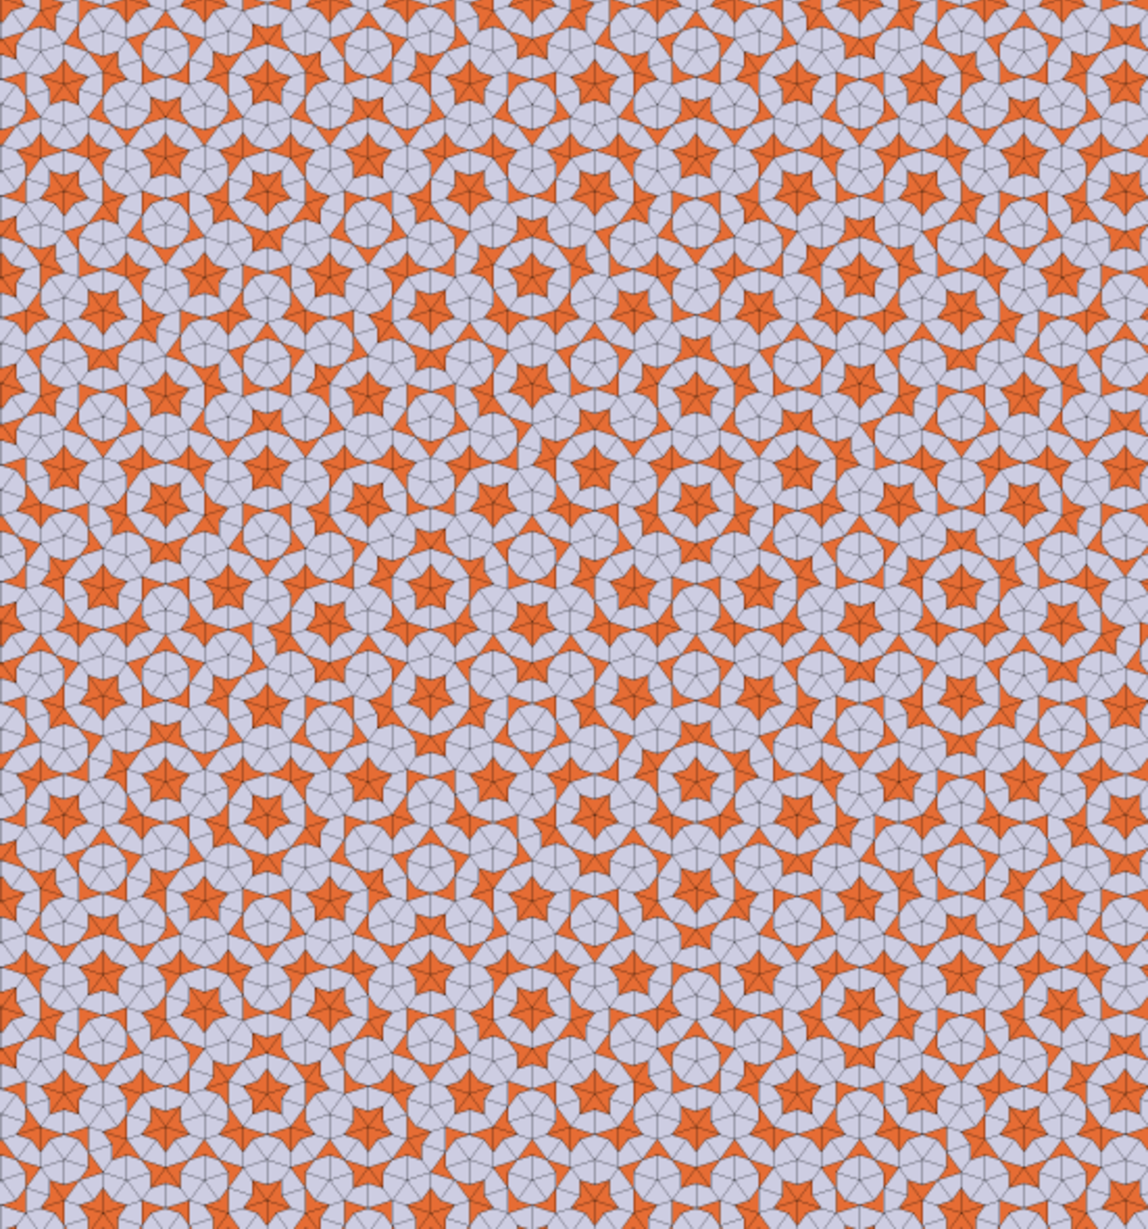
\includegraphics[width=2.5in]{./figs/penrose.pdf} 
   \caption{Penrose kite and dart tiling from the Tilings Encyclopedia Website (\texttt{http://tilings.math.uni-bielefeld.de/substitution$\empty\_$rules/})}
   \label{fig:example}
\end{figure}

